\chapter{Résultats}
\section{Modes}
\label{resModes}

\subsection{Valeurs analytiques de $\lambda$}

D'après \cite{Saks2005}, on a, pour un cylindre de longueur $l$ et de rayon $R$ :
\[
\lambda_\mathcal{K} = \sqrt{\frac{\rho_{k,j}^2}{R^2} + \frac{m^2\pi^2}{l^2}}
\]
où $\mathcal{K}=(k,j,m)$ est un multi-index et $\rho_{k,j}$ représente le j-ième zéro de la k-ième fonction de Bessel.\\
Dans notre cas, $l=0,5$ et $R=0,05$, d'où :\\
\begin{center}
\begin{tabular}{|*{8}{c|}}
\hline
k & j & m=1 & m=2 & m=3 & m=4 & m=5 & m=6\\
\hline
\multirow{3}{*}{0}
& 1 & 2352,703634&2471,138886&2668,530974&2944,879898&3300,185656&3734,44825\\
& 2 & 12228,08002&12346,51527&12543,90736&12820,25629&13175,56204&13609,82464\\
& 3 & 29994,08789&30112,52315&30309,91523&30586,26416&30941,56992&31375,83251\\
\hline
\multirow{3}{*}{1}
& 1 &5912,248374&6030,683626&6228,075714&6504,424638&6859,730396&7293,99299\\
& 2 &19726,93576&19845,37101&20042,7631&20319,11203&20674,41778&21108,68038\\
& 3 &41439,51932&41557,95457&41755,34666&42031,69558&42387,00134&42821,26393\\ \hline
\multirow{3}{*}{2}
& 1 &10589,23336&10707,66861&10905,0607&11181,40963&11536,71538&11970,97798\\
& 2 &28379,18075&28497,61601&28695,00809&28971,35702&29326,66278&29760,92537\\
& 3 &54047,37923&54165,81449&54363,20657&54639,5555&54994,86126&55429,12385\\
\hline
\multirow{3}{*}{3}
& 1 &16322,25923&16440,69449&16638,08657&16914,4355&17269,74126&17704,00385\\
& 2 &38150,32682&38268,76207&38466,15416&38742,50308&39097,80884&39532,07143\\
& 3 &67797,65083&67916,08609&68113,47817&68389,8271&68745,13286&69179,39545\\
\hline
\multirow{3}{*}{4}
& 1 &23072,39717&23190,83243&23388,22451&23664,57344&24019,8792&24454,14179\\
& 2 &49010,51285&49128,94811&49326,34019&49602,68912&49957,99488&50392,25747\\
& 3 &82666,98092&82785,41617&82982,80826&83259,15718&83614,46294&84048,72553\\
\hline
\end{tabular}
\end{center}

Il montre aussi que :
\[
g_\mathcal{K}^z(r,\theta,z) = \frac{\sqrt{2}}{\sqrt{l\pi}R|J_k'\left(\rho_{k,j}\frac{r}{R}\right)}exp(ik\theta)sin\left(\frac{m\pi}{l}z\right)
\]

\iffalse

Pour mémoire, voici les résultats de différents modes obtenus avec freefem++.\\

\begin{figure}[H]
\makebox[\textwidth][c]{
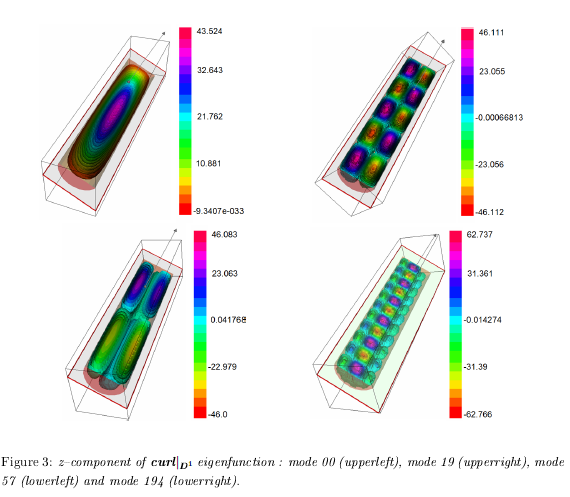
\includegraphics[scale=1]{Exemple_de_modes}}
\end{figure}

On peut voir les mêmes modes obtenus avec Feel++ dans la figure \ref{modes}.\\

\begin{figure}[H]
	\makebox[\textwidth][c]{
		\subfloat[mode00]{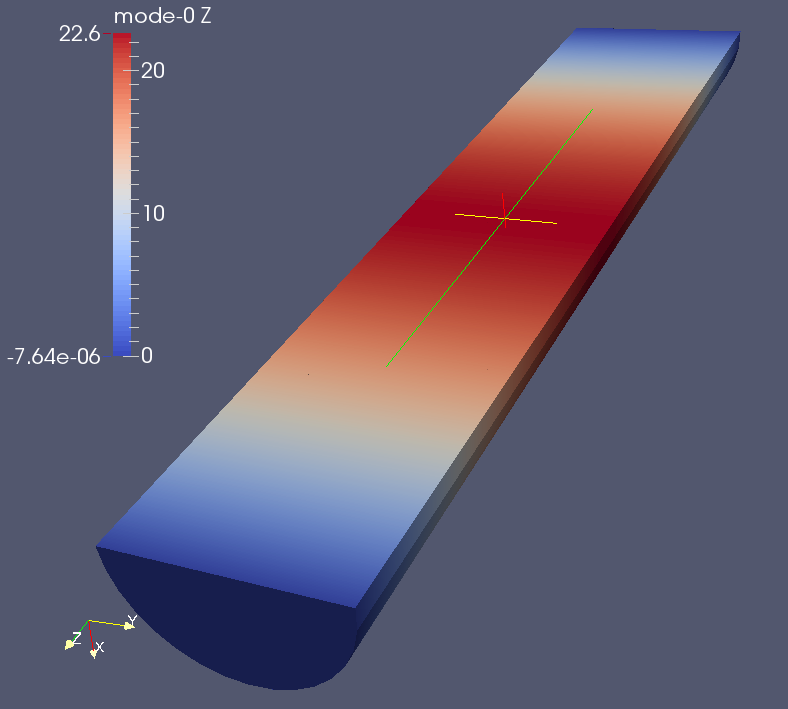
\includegraphics[scale=0.3]{mode00}}\ 
		\subfloat[mode19]{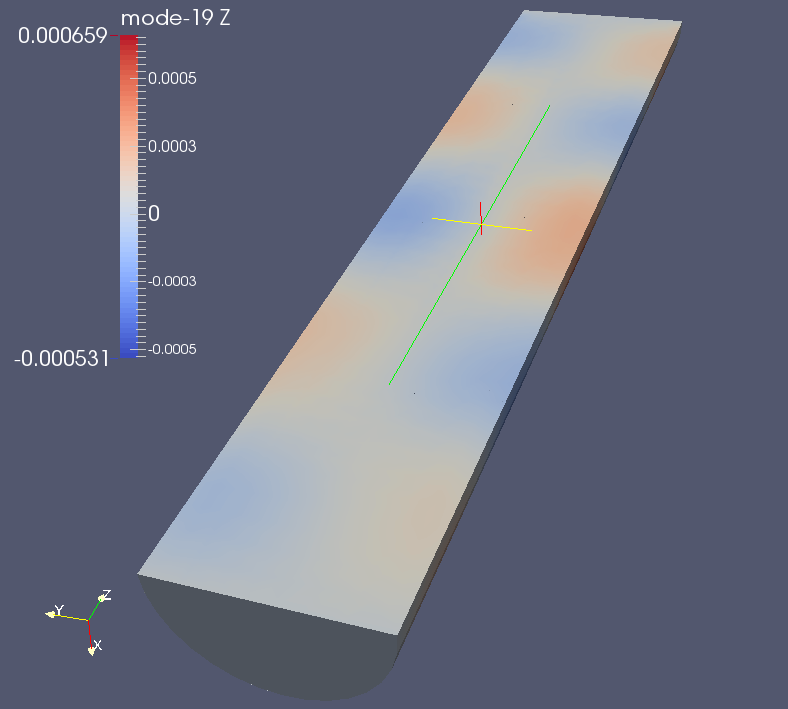
\includegraphics[scale=0.3]{mode19}}
	}\\
	\makebox[\textwidth][c]{
		\subfloat[mode57]{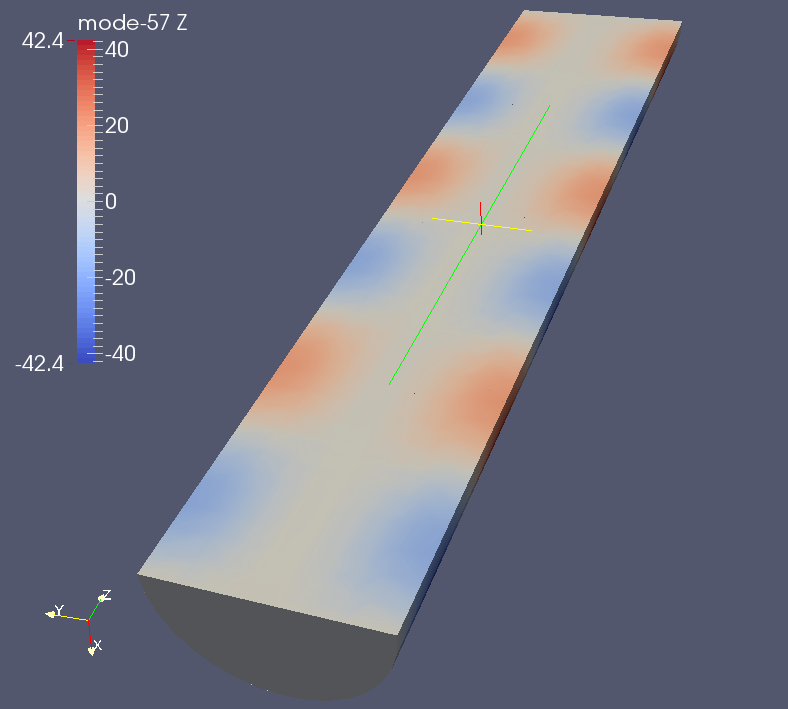
\includegraphics[scale=0.3]{mode57}}\ 
		\subfloat[mode194]{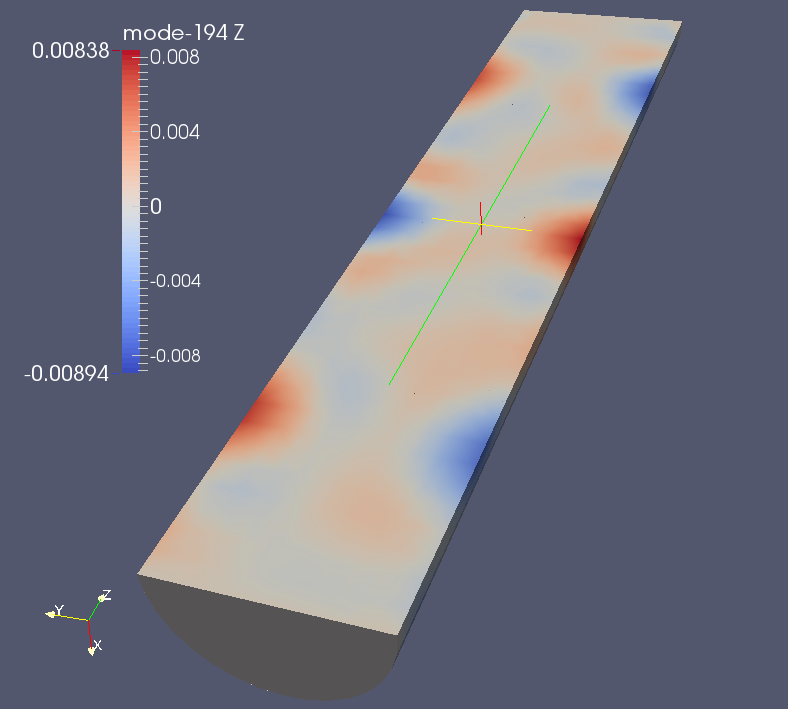
\includegraphics[scale=0.3]{mode194}}
	}
	\caption{composante z des fonctions propres}
	\label{modes}
\end{figure}

\fi

\subsection{Composante z}

En utilisant l'implèmentation présenté dans la section \ref{compZ}, on obtient les valeurs propres suivantes, où l'on voit que les valeurs propres ne correspondant pas à la fonction 0 de Bessel, apparaissent deux fois, cela est dû à la symétrie du cylindre.\\
D'autre part, on voit qu'à partir d'un certain moment, les valeurs propres ne correspondent plus aux valeurs analytiques et que leur divergence explosent.\\

\begin{align*}
\bm{\lambda^2_{0,1,1}=\Lambda_0} &\bf{= 2329.47}	&\int\div\bm{g} &= 1.94208e-17	&||\div\bm{g}|| &= 0.0983456\\
\lambda^2_{1,1,1}=\Lambda_1 &= 5917.22	&\int\div\bm{g} &= 3.17129e-18	&||\div\bm{g}|| &= 0.296662\\
\lambda^2_{1,1,1}=\Lambda_2 &= 5917.43	&\int\div\bm{g} &= -3.4708e-17	&||\div\bm{g}|| &= 0.299039\\
\lambda^2_{2,1,1}=\Lambda_3 &= 10644.7	&\int\div\bm{g} &= 2.20627e-17	&||\div\bm{g}|| &= 0.683934\\
\lambda^2_{2,1,1}=\Lambda_4 &= 10647.4	&\int\div\bm{g} &= 2.89804e-17	&||\div\bm{g}|| &= 0.688444\\
\bm{\lambda^2_{0,2,1}=\Lambda_5} &\bf{= 12312.1}	&\int\div\bm{g} &= -1.04863e-16	&||\div\bm{g}|| &= 0.954444\\
\lambda^2_{3,1,1}=\Lambda_6 &= 16473	&\int\div\bm{g} &= -1.28681e-17	&||\div\bm{g}|| &= 1.23079\\
\lambda^2_{3,1,1}=\Lambda_7 &= 16474.4	&\int\div\bm{g} &= -2.9924e-17	&||\div\bm{g}|| &= 1.22237\\
\lambda^2_{1,2,1}=\Lambda_8 &= 19976.6	&\int\div\bm{g} &= -5.4515e-17	&||\div\bm{g}|| &= 1.8095\\
&\vdots & &\vdots & &\vdots\\
\lambda^2_{?,?,?}=\Lambda_{35} &= 51355.4	&\int\div\bm{g} &= 1.14817e-16	&||\div\bm{g}|| &= 7.14748\\
\lambda^2_{?,?,?}=\Lambda_{36} &= 54891.3	&\int\div\bm{g} &= 1.21431e-17	&||\div\bm{g}|| &= 50.2826\\
\lambda^2_{?,?,?}=\Lambda_{37} &= 55565.9	&\int\div\bm{g} &= -2.43729e-16	&||\div\bm{g}|| &= 52.281\\
\lambda^2_{?,?,?}=\Lambda_{38} &= 55976.2	&\int\div\bm{g} &= -1.73906e-16	&||\div\bm{g}|| &= 58.8682\\
\lambda^2_{?,?,?}=\Lambda_{39} &= 56447.3	&\int\div\bm{g} &= 1.50813e-16	&||\div\bm{g}|| &= 59.4463\\
\lambda^2_{?,?,?}=\Lambda_{40} &= 57302.4	&\int\div\bm{g} &= 4.13081e-17	&||\div\bm{g}|| &= 40.4527\\
\lambda^2_{?,?,?}=\Lambda_{41} &= 57360.6	&\int\div\bm{g} &= -3.61581e-17	&||\div\bm{g}|| &= 36.7049\\
\lambda^2_{?,?,?}=\Lambda_{42} &= 57614.4	&\int\div\bm{g} &= -8.2833e-17	&||\div\bm{g}|| &= 44.0287\\
\lambda^2_{?,?,?}=\Lambda_{43} &= 57825.8	&\int\div\bm{g} &= 1.47451e-16	&||\div\bm{g}|| &= 58.9588\\
\lambda^2_{?,?,?}=\Lambda_{44} &= 58151.4	&\int\div\bm{g} &= -9.36751e-17	&||\div\bm{g}|| &= 62.1296\\
\lambda^2_{?,?,?}=\Lambda_{45} &= 59027	&\int\div\bm{g} &= 1.70328e-16	&||\div\bm{g}|| &= 54.9454\\
\lambda^2_{?,?,?}=\Lambda_{46} &= 59732.7	&\int\div\bm{g} &= -1.66371e-16	&||\div\bm{g}|| &= 37.642
\end{align*}

Les modes correspondant aux trois premiers zéros de la fonction 0 de Bessel sont présenté dans la figure suivante, avec un autre mode où l'on voit que ces fonctions ne dépendent pas de $\theta$ contrairement aux autres :
\begin{figure}[H]
	\makebox[\textwidth][c]{
		\subfloat[mode 0]{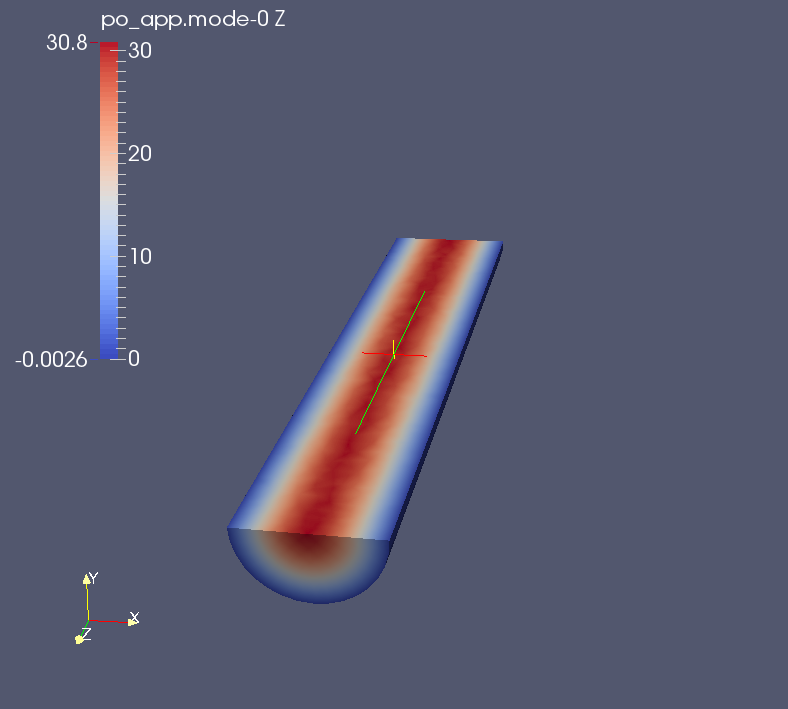
\includegraphics[scale=0.3]{modeZ-0}}\ 
		\subfloat[mode 5]{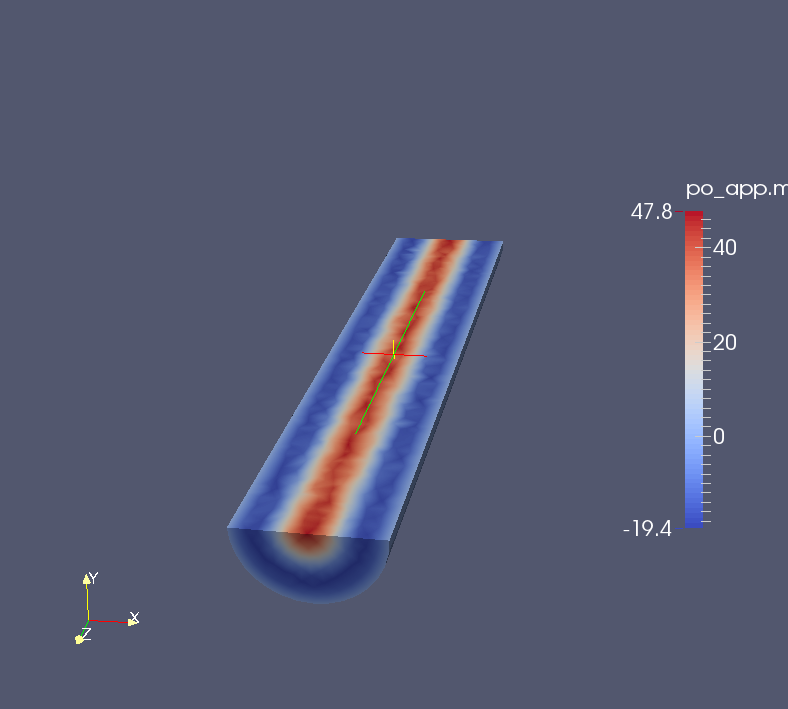
\includegraphics[scale=0.3]{modeZ-5}}
	}\\
	\makebox[\textwidth][c]{
		\subfloat[mode 14]{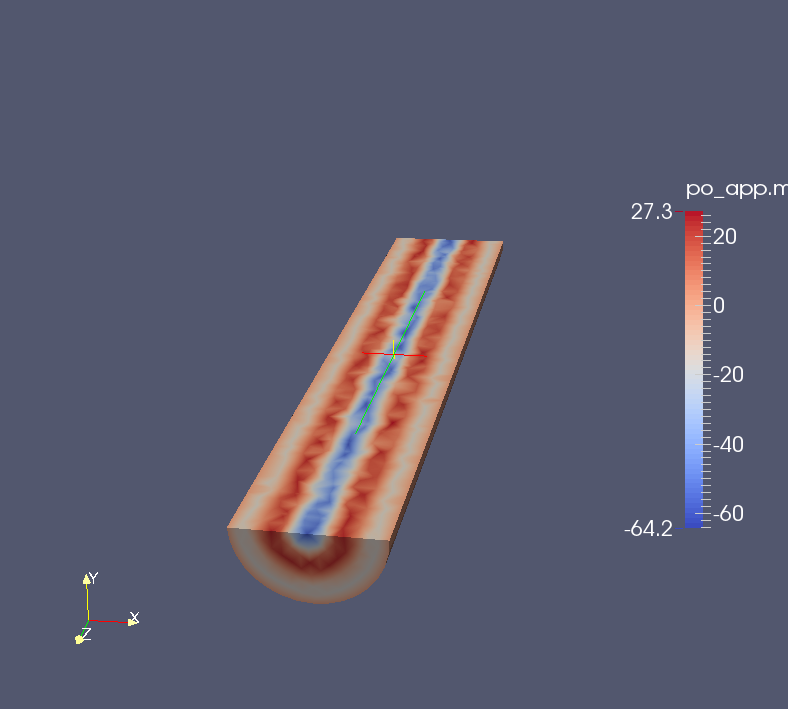
\includegraphics[scale=0.3]{modeZ-14}}\ 
		\subfloat[mode 16]{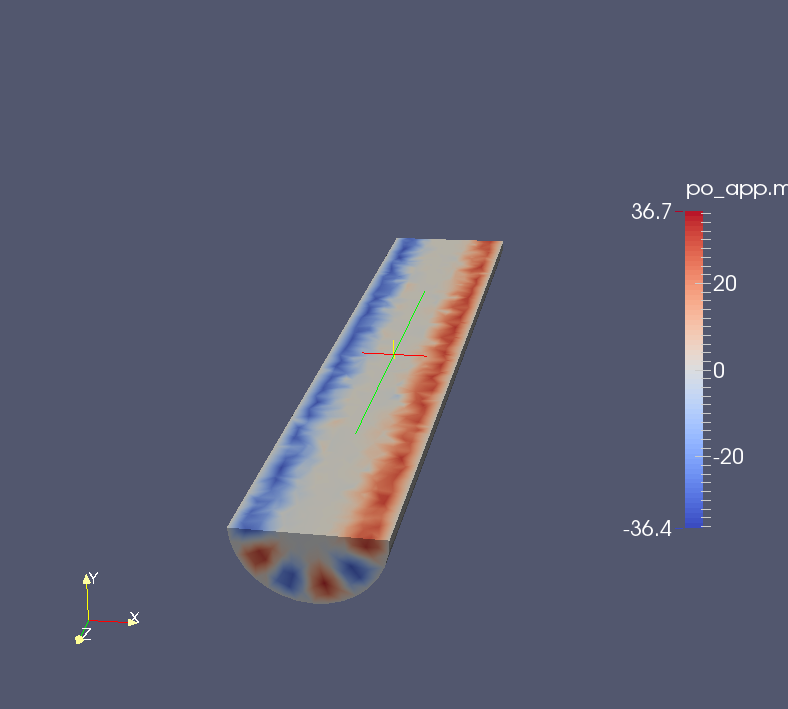
\includegraphics[scale=0.3]{modeZ-16}}
	}
	\caption{composante z des fonctions propres}
	\label{resultats}
\end{figure}


\section{Relèvement}
\label{respsih1}

Dans la figure \ref{az}, on peut observer la composante en $z$ de $\mathbf{a}$ dans le cylindre, lorsque $\alpha_1=0$ et $\alpha_0(x,y)=2\times v\times\left(1-\frac{x^2+y^2}{r^2}\right)$. Ce résultat a été obtenu avec le programme du chapitre \ref{gradh1}. 

\begin{figure}[H]
\makebox[\textwidth][c]{
  \subfloat{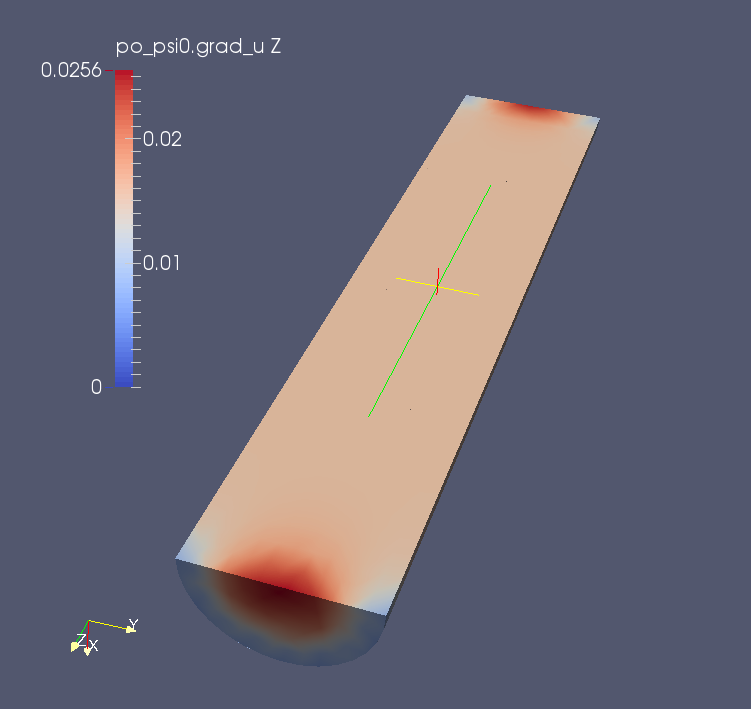
\includegraphics[scale=0.3]{az}}\ 
  \subfloat{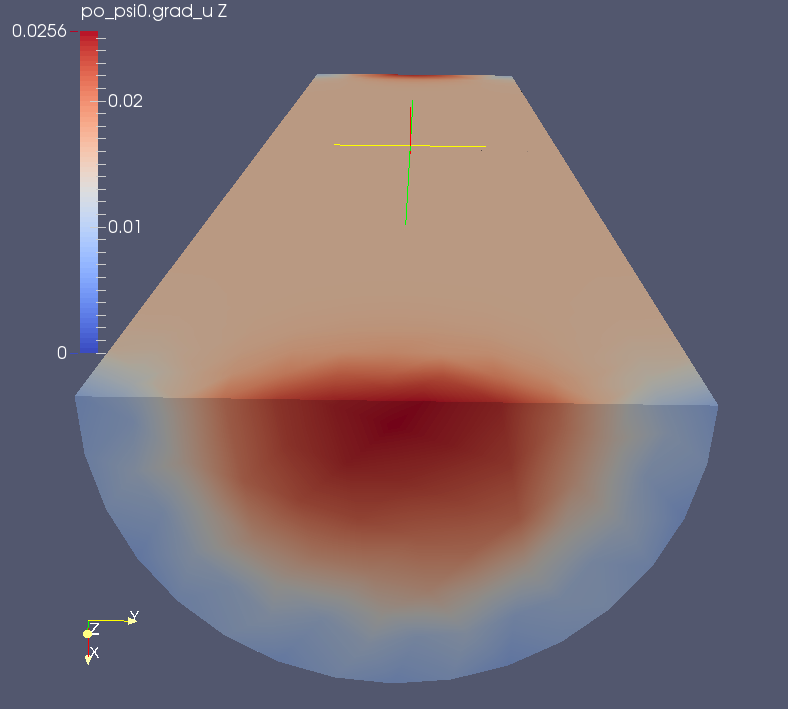
\includegraphics[scale=0.3]{az1}}
}
\caption{$\mathbf{a}=\grad\psi^0\in H(div)$}
\label{az}
\end{figure}

%%% Local Variables:
%%% TeX-master: "../report.tex"
%%% End:
